\subsection{Aprendizagem profunda}

A aprendizagem profunda é uma subcategoria do aprendizado de máquinas \cite{lecun2015deep}.
Semelhante ao aprendizado de máquina, o aprendizado profundo também possui aprendizado supervisionado, não-supervisionado e de reforço.
O algoritmo de aprendizagem profunda depende de redes neurais profundas. 
Redes neurais profundas podem automaticamente achar representações compactas de baixa dimensionalidade de dados com alta dimensionalidade (e.g., imagens, texto e audio) \cite{arulkumaran2017brief}.
Essas redes neurais foram baseadas no funcionamento dos neurônios do cérebro humano. 
Ou seja, o aprendizado profundo vem dá criação de redes neurais que possuem neurônios que se comunicam entre si e conseguem passar informação. 

Uma Rede Neural Profunda (DNN) consiste de múltiplas camadas de unidades de processamento não-linear (camada escondida). Ela executa a extração e transformação de características. Na Figura \ref{fig:NN} é mostrada uma DNN que consiste que três camadas: camada de entrada, camadas escondidas e camada de saída. Na camada de entrada, os neurônios são generalizados a partir de recursos que passam por sensores que percebem o ambiente. As camadas escondidas podem incluir uma ou mais camadas. A camada de saída contem a saída desejada, por exemplo, a distribuição de todas as ações possíveis.
Cada camada sucessiva da DNN usa a saída da camada anterior como entrada.
Todos os neurônios das camadas são totalmente ativados através de conexões ponderadas.

\vspace{0.25cm}
\begin{figure}[H]
\caption{Rede Neural Simples e Profunda}
\centerline{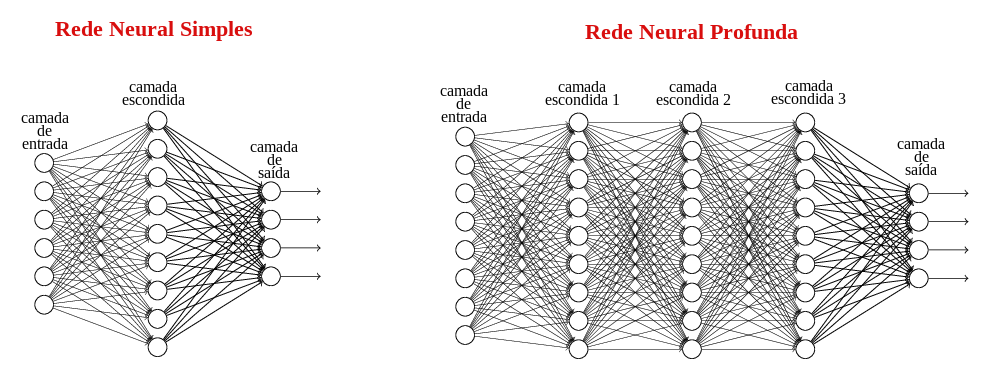
\includegraphics[width=\columnwidth]{imagens/neural_network.png}}
\small{Fonte: http://neuralnetworksanddeeplearning.com/chap5.html}
\label{fig:NN}
\end{figure}

Todas as DNN são funções matemáticas. 
Então, para calcular a função de uma camada é usado a definição abaixo:
\begin{equation}
    a^{(c)} = W a^{(c-1)} + b
    \label{eq:camada}
\end{equation}

Sendo os neurônios da camada atual $a^{(c)}$ e da camada anterior $a^{(c-1)}$, os pesos de todas as conexões entre as duas camadas $W$ e um número pré-determinado de bias $b$.

Contudo, em aplicações do mundo real, funções lineares não conseguem descrever todos os sistemas, quase sempre, funções não-lineares são usadas. Para fazer isso é preciso aplicar uma função não-linear, conhecida como função de ativação (FA), a Equação \ref{eq:camada}, que ficaria definida como:
\begin{equation}
    a^{(c)} = FA\left\{W a^{(c-1)} + b\right\}
\end{equation}

Então, para resolver sistemas não-lineares diferentes funções de ativação podem ser usadas ou pode ser criada a própria função de ativação que se ajusta ao problema. Existem diversas FA's pré-definidas, tais como: `linear', `ReLU', `tanh', `sigmoid', etc.
Na Figura \ref{fig:FA} é mostrada a respostas para as FA's mais conhecidas.

\begin{figure}[H]
\caption{Exemplos de resposta de funções de ativação}
\centerline{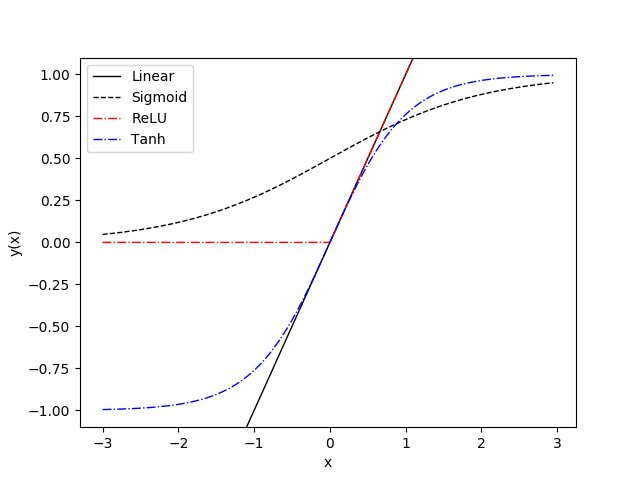
\includegraphics[width=\columnwidth]{imagens/function_activation.png}}
\small{Fonte: Autor}
\label{fig:FA}
\end{figure}

Depois do fluxo de computação avançar da entrada para a saída, na camada de saída e cada camada escondida, é possível calcular o erro derivativo para propagar os gradientes em direção a camada de entrada, sendo assim os pesos podem ser atualizados para otimizar a função de perda \cite{li2017deep}. Isto é o foco da parte de aprendizagem, para achar os pesos e bias certos.

% Geralmente utiliza-se de redes neurais e de muitos dados para o seu treinamento. 
% Essas redes neurais foram baseadas no funcionamento dos neurônios do cérebro humano. Ou seja, o aprendizado profundo vem dá criação de redes neurais que possuem neurônios que se comunicam entre si e conseguem passar informação. 
% E enquanto, programas tradicionais constroem análises com dados de uma forma linear, o aprendizado profundo constrói funções hierárquicas para o processamento de dados de uma forma não linear.

% Uma rede neural, na sua forma mais simples, é composta de múltiplas camadas de nós interconectados, como é mostrado na Figura 3. 
% As conexões da rede são similares as conexões dos neurônios do cérebro humano. 
% A conexão entre as camadas possuem um nó e a este nó está associado a um peso. 
% A rede neural é treinada pelo uso de grandes conjuntos de dados rotulados que aprendem características diretamente dos dados sem a necessidade da intervenção manual.

% figura

% A rede neural pode apresentar um maior número de camadas escondidas assim podendo-se classificar como uma rede “profunda”.
% Em uma rede neural com múltiplas camadas escondidas, o número de parâmetros cresce exponencialmente, podendo assim ter uma melhor eficiência para a resolução de problemas que uma rede neural de apenas uma única camada escondida.

% Muitos dos modelos modernos de aprendizado profundo são baseados em uma rede neural artificial. Cada nível da rede aprende a transformar as informações de entrada em algo  mais abstrato. 
% Como regra, quanto mais profunda é o modelo, mais a rede tem potencial de obter um melhor desempenho que os modelos mais superficiais. 
% O problema é que quanto mais profunda é a rede, mais dados são necessários para evitar o sobreajuste, sem falar, do aumento do tempo para obter uma resposta de saída.
% No caso de uma rede que vá cuidar de um robô, em constante movimento, é preciso ter uma resposta mais rápida. Logo, uma rede superficial é melhor para esse tipo de aplicação.